\chapter{Antecedentes}

\section{Fenómeno de la fatiga y su medición}
El fenómeno en el cual una estructura se daña e incluso falla por cargas fluctuantes, es llamado fatiga. El estudio de este problema comenzó tempranamente en Europa durante la mitad del siglo XIX, en pleno auge de la industralización europea, producto de la falla repentina de algunos componentes en máquinas y los ejes de los trenes de la época. Estos experimentaban un gradual debilitamiento de la resistencia, fallando aún cuando su esfuerzo último no fuese alcanzado. 

Así, en 1837 fueron publicados los resultados del primer ensayo de fatiga, realizado a una cadena transportadora utilizada en minas de hierro en Alemania. Wilhelm Albert, quien realizó esta investigación, se vio motivado a realizar los estudios por los altos costos que significaba la falla de este componente producto de las cargas cíclicas a las que estaba sometida. Los pocos conocimientos existentes del fenómeno en aquella época, llevaron a que la solución al problema fuese la invención del cable de acero.

Por otro lado, las primeras investigaciones enfocadas a comprender el fenómeno comenzaron en 1858 con August Wölher. Su acucioso estudio lo llevó a conclusiones que siguen teniendo importancia y validez hasta el día de hoy. Diseñó, durante la década de 1860, una máquina de ensayos de flexión y flexión rotativa. En 1870 presentó un informe en el cual parte de sus conclusiones cualitativas son llamadas ``Ley de Wöhler'', al establecer el esfuerzo alternante como el parámetro más importante para la vida de un componente, señalanado que: ``the stress amplitudes are decisives for the destruction of the cohesion of the material. The maximum stress is of influence only in so far as the higher it is, the lower are the stress amplitudes which lead to failure''\cite{schutz1996history}. Se destaca también que el esfuerzo medio tiene una influencia perjudicial en el material. 

Es decir, desde 1853 hasta hoy, han transcurrido más de 160 años de investigación sobre la fatiga, logrando comprender distintas aristas del fenómeno, pero con muchas preguntas aún sin resolver. Por lo tanto, la fatiga sigue siendo un problema necesario de abordar y seguir comprendiendo por sus grandes implicaciones de costo que tiene en la industria y en los distintos elementos que utilizamos en la vida diaria. Por otro lado, si bien muchas preguntas no han sido resueltas científicamente, diversas empresas han logrado evitar las fallas por fatiga y optimizar los diseños de manera operativa, sin comprender cabalmente el trasfondo de estos.

\subsection{Medición de la fatiga}
Existen distintas técnicas para cuantificar la respuesta de un material o componente frente a esfuerzos o deformaciones fluctuantes. La primera de ellas, como se habló anteriormente, corresponde a una viga giratoria sometida a flexión en voladizo diseñada por A. Wöhler. Con respecto a la información existente en la literatura, la mayoría de los datos disponibles de resistencia a la fatiga se encuentra en las pruebas de viga giratoria (\textit{rotating bending}, en inglés) en ciclo de flexión invertida, seguido por cargas axiales (\textit{push-pull}, en inglés), flexión en voladizo o flexión alternante (\textit{alternating bending}, en inglés) y en menor medida, en las pruebas de fatiga por torsión. \cite{norton2011machine}

\begin{figure}[h]
\centering
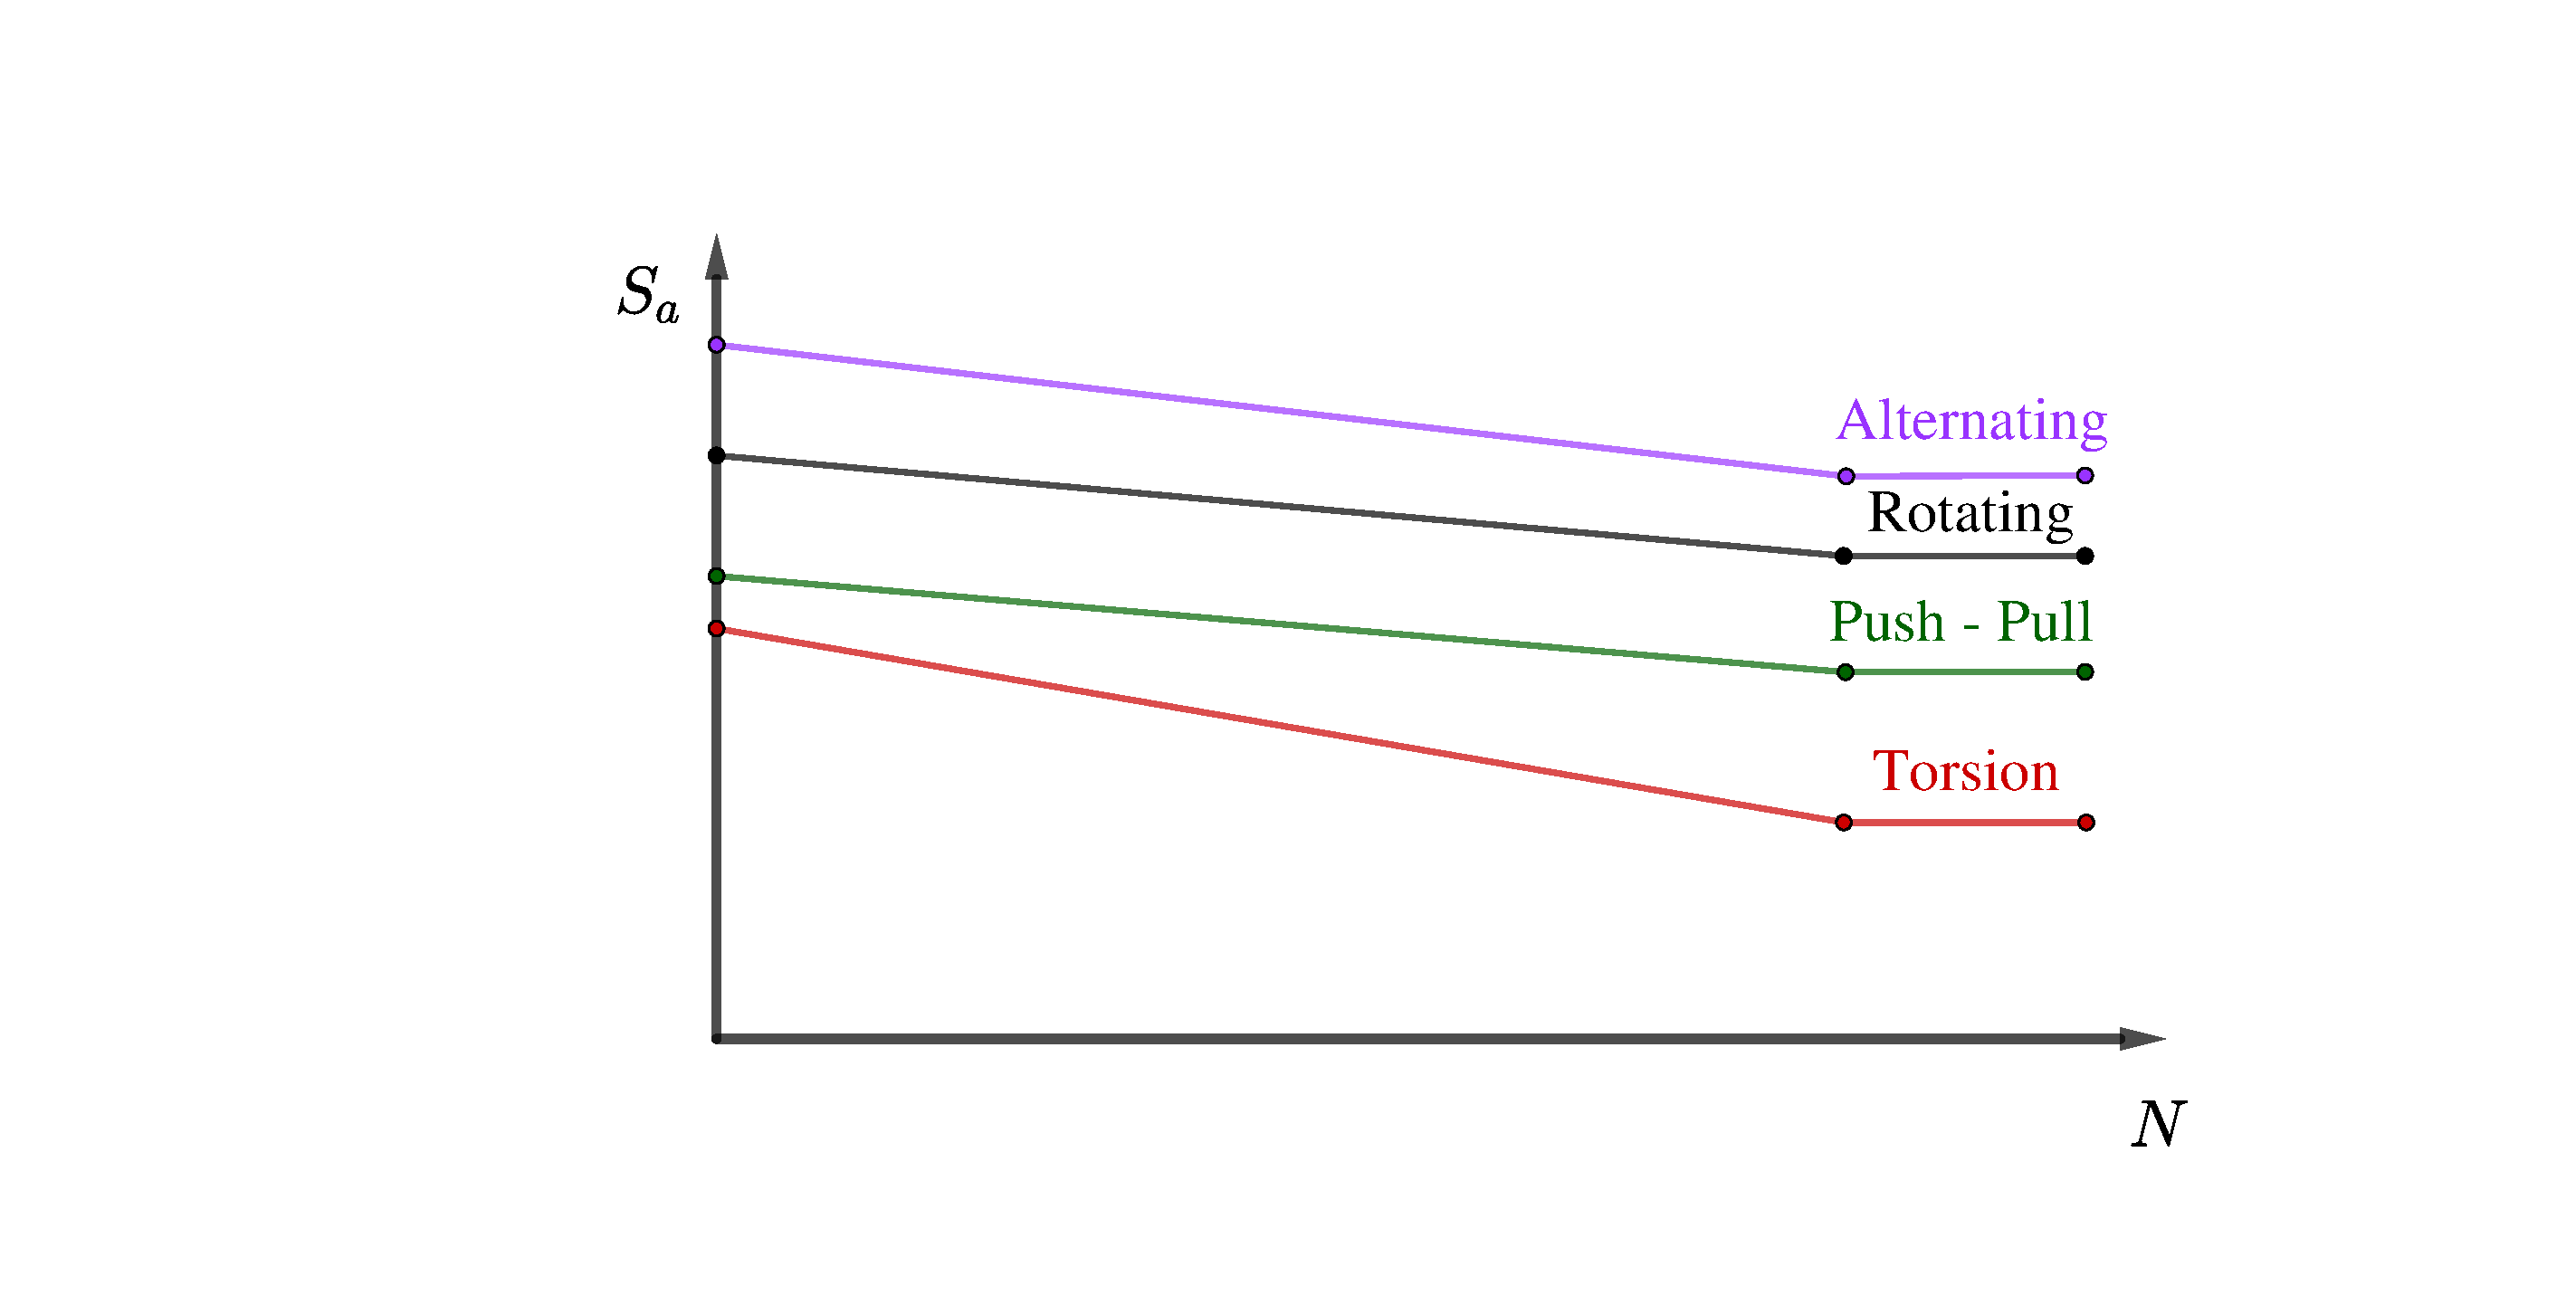
\includegraphics[width=0.9\linewidth, trim={11cm 2cm 6cm 4cm}, clip]{Imagenes/comp_medfat.pdf}
\caption{Comparación entre las distintas curvas caracterísitcas de cada forma de medición de la fatiga para el acero. \cite{lee2005fatigue}\cite{esin1980method}}
\label{fig:comp_medfat}
\end{figure}


\subsubsection{Ensayo de fatiga con una viga giratoria en flexión} 
Su uso es el más extendido para determinar la vida a fatiga de un material. La principal ventaja frente a otros sistemas radica en su capacidad de aplicar ciclos de cargas a altas velocidades, es decir, realizar pruebas de fatiga a altas frecuencias. Sin embargo, no es posible aplicar una carga media distinta de cero, por lo tanto, su uso principal se encuentra en la obtención de datos para un régimen de fatiga de alto ciclaje y de ciclo invertido. Los datos obtenidos de la resistencia a la fatiga son inferiores a los obtenidos por medio de flexión alternante, como se puede ver en la fig. \ref{fig:comp_medfat}.


\subsubsection{Ensayo de fatiga axial}
Esta configuración de prueba es más flexible que el resto, siendo posible cualquier combinación de esfuerzo alternante y medio 	\cite{norton2011machine}. Su principal diferencia respecto al método de viga giratoria se encuentra en que la sección transversal está sometida a esfuerzos de manera uniforme, provocando que los resultados de resistencia a la fatiga obtenidos sean usualmente menores a aquellos obtenidos por viga giratoria y flexión alternante. Se considera que esto se debe a la  probabilidad más alta de hallar una micro-grieta en un campo de esfuerzos más grande. Asimismo, la superposición de momentos de flexión sobre las cargas axiales, producto de la dificultad de crear cargas axiales sin excentricidad, son un factor en la disminución en la obtención de valores de resistencia menores. En concreto, la reducción de la resistencia a la fatiga obtenidas pueden variar entre un 10$\%$ y un 30$\%$ o más si hay flexión producto de la excentricidad de las cargas \cite{bannantine1990fundamentals}. La fig. \ref{fig:comp_medfat} muestra las diferencias de los datos obtenidos entre un ensayo de fatiga axial y el resto de las formas de medición.

\subsubsection{Ensayo de fatiga de flexión en voladizo o flexión alternante}
Esta prueba consiste en someter a una viga en voladizo a oscilaciones en su extremo libre a través de algún mecanismo, pudiendo lograr combinaciones de esfuerzos medios y alternantes. La máquina analizada en esta memoria utiliza este método para la obtención de los datos de vida de fatiga del material a analizar. Los resultados de este tipo de prueba son los más altos respecto a otros tipos de medición de fatiga.

\subsection{Correlación entre distintos métodos de medición de la fatiga}
Como se señaló anteriormente y se aprecia en la fig. \ref{fig:comp_medfat}, cada prueba entrega valores distintos aún cuando los niveles de esfuerzo sean iguales. Por esto, existen distintos intentos en la literatura de crear correlaciones entre los datos, evitando los costos asociados a realizar nuevos ensayos experimentales del mismo material o componente. La forma en que se ha abordado esta problemática es la utilización de un factor de corrección ($\phi$) calculado con distintas propuestas.

Algunos de estos modelos son: Philipp, Lee, Esin y Manson y Muralidharan. Cada metodología aborda de distinta forma el cálculo del factor de corrección $\phi$, ahora bien, se abordarán los modelos de Lee y Esin en este trabajo, ya que son los modelos que se ajustan mejor al comportamiento de los datos empíricos de ensayos de fatiga. \cite{strzelecki2018analysis}

\subsubsection{Modelo de Esin}
El modelo propuesto por Esin \cite{esin1980method} relaciona las curvas $S$-$N$ de los ensayos fatiga axial, flexión alternante y flexión rotativa. Éste depende de la micro-plasticidad, determinada por el esfuerzo alternante y su distribución en la sección transversal \cite{strzelecki2018analysis}. 

Este método se basa en estudios previos del mismo autor, los cuales buscan entender y predecir el fenómeno de la fatiga a través de las propiedades mecánicas de un material. Para esto, proponen una teoría de fatiga basada en la acumulación micro-estructural de la energía de deformación \cite{esin1966theory}, mediante la cual establecen que la micro-inhomogeneidad de las propiedades mecánicas, así como del estado de esfuerzos, está relacionada con la vida a fatiga de un material.

La fatiga, a niveles de alto ciclaje, es un fenómeno localizado, fuertemente influenciado por su micro-estructura, anisotría, inclusiones, su estructura cristalina, granos u otros, los cuales explican la dispersión de datos en los ensayos de fatiga \cite{esin1968microplastic}. En consecuencia, la fatiga está asociada con el deslizamiento plástico que ocurre a un nivel micro-estructural cuando el material es nominalmente elástico. Se le denomina micro-plasticidad por ocurrir a nivel de la micro-estructura y ocurre sobre cierto nivel de esfuerzos en el rango elástico llamado límite elástico real (\textit{true elastic limit}, en inglés o \textit{TEL}). Este se encuentra siempre por debajo del límite de resistencia a la fatiga ($S_e$), lo que da como resultado:
\begin{align*}
	\text{\textit{TEL}} \leq S_e \leq S_y
\end{align*}
Así, cuando los esfuerzos alternantes están sobre valor del  \textit{TEL}, la micro-plasticidad influye en los macro-elementos. Dicho de otra forma, el comportamiento mecánico observado a un nivel macro es el comportamiento integrado de los micro-elementos.

La micro-plasticidad es analizada de manera probabilística, calculando el número de micro-elementos en plasticidad que se encuentran en el área transversal sometida a fatiga. El área afectada para cada tipo de ensayo se puede apreciar en la fig. \ref{fig:affar_fat}.

\begin{figure}[h]
\centering
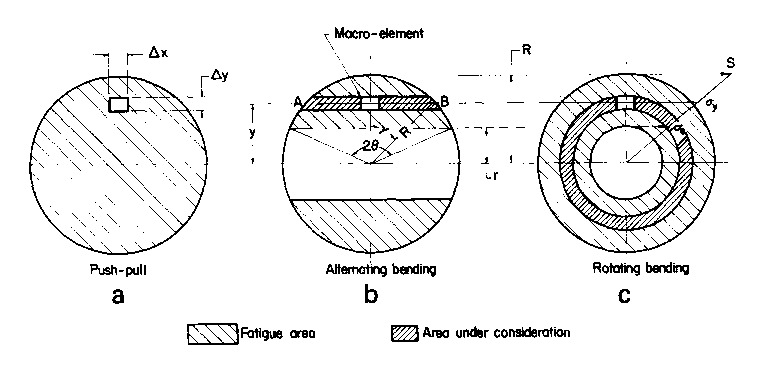
\includegraphics[scale=1]{Imagenes/affectedarea_fatigue.pdf}
\caption{Sección transversal de probetas sujetas a esfuerzo alternante uniaxial. \textit{a) push-pull}, \textit{b) alternating bending} y \textit{c) rotating bending}. \cite{esin1980method}}
\label{fig:affar_fat}
\end{figure}

De esta manera, el autor sostiene que el daño por fatiga está relacionado a la acumulación, a nivel micro-estructural, de la energía de histéresis plástica y, por lo tanto, se afirma que la falla del material ocurre cuando la energía acumulada por la histéresis plástica es igual a la energía requerida para la fractura en tracción, determinada como el área bajo la curva de un diagrama de esfuerzo-deformación real ($U_{rup}$). Por lo tanto, se puede estudiar el daño de la fatiga en términos de la energía de deformación micro-plástica disipada por cada ciclo de una carga ($\Omega$) \cite{esin1967stress}. El número total de ciclos a la fractura es:
\begin{gather}
	N_f = \frac{U_{ruptura}}{\Omega}
\end{gather} 

Si para cada tipo de ensayo de fatiga se utiliza una probeta de igual geometría y dimensión, sometidas al mismo esfuerzo alternante promedio, la energía plástica disipada por cada ciclo no serán igual producto de las distintas áreas afectadas por fatiga, como se muestra en la fig. \ref{fig:affar_fat}. Para esto, el método utiliza los conceptos de esfuerzo alternante equivalente y vida a fatiga equivalente, los cuales se relacionan mediante puntos ($S$,$N$) de la curva de fatiga, la proporción entre el área total transversal y el área que contribuye a la fatiga y la distribución de esfuerzos dentro del área afectada, para entregar un punto ($S'$,$N'$) de la curva buscada. Este procedimiento se debe repetir de manera iterativa hasta conseguir ajustar los puntos a una curva.

\subsubsection{Modelo de Lee}
La estimación del límite de fatiga, $S_e$, se calcula a través de distintos factores de modificación según el tipo de carga, calidad superficial, tamaño y confiabilidad de la muestra. El factor de modificación según el tipo de carga $C_L$ varía entre 0,7 y 0,9 para probetas sin muescas. Las recomendaciones para cada valor de $C_L$ se realizaron considerando los efectos del gradiente de esfuerzos y el tipo de esfuerzo involucrado, es decir, cortantes y normales. Estos también varían según el tipo de material, los cuales fueron obtenidos de manera empírica. Así la tabla \ref{tab:lee_factor} muestra los factores de modificación para algunos tipos de carga.

\begin{table}[h]
\centering
\caption{Factores de modificación por tipo de carga, según el modelo de Lee.}
\begin{tabular}{@{}llc@{}}
\toprule
Tipo de Carga                & $C_L$ & Observaciones \\ \midrule
Carga axial pura             & 0,9   & -                                 \\
Carga axial con leve flexión & 0,7   & -                                 \\
Rotating bending             & 1,0   & -                                 \\
Torsional                    & 0,58  & Para aceros   \\ \bottomrule
\end{tabular}
\label{tab:lee_factor}
\end{table}

\subsubsection{Comparación entre ambos modelos}

Ambos métodos toman en consideración distintos elementos y utilizan distintas formas para desarrollar sus resultados. El primero de ellos, el método de Esin es consecuencia del desarrollo de una teoría que busca predecir el comportamiento a fatiga a partir del estudio las propiedades micro-estructurales \cite{esin1966theory}, buscando darle una base física al desarrollo de la metodología. Sin embargo, si bien el método es eficaz \cite{strzelecki2018analysis}, está limitado por no considerar los cambios de geometría ni dimensiones y por la necesidad de tener información sobre la micro-estructura del material y el límite elástico real. Por otro lado, el método de Lee utiliza la información recolectada de distintos ensayos, generando correlaciones empíricas entre las distintas curvas \cite{lee2005fatigue}. Esto, trae como consecuencia la poca flexibilidad del método, al ser dependiente de que exista información previa sobre un material en particular y de los ensayos buscados.

\newpage

\section{Máquina de fatiga a flexión}
El desarrollo de este trabajo se centrará en la máquina de fatiga que posee el departamento de ingeniería mecánica en el laboratorio de tecnología mecánica en Valparaíso. La información existente sobre la máquina de ensayo es escasa principalmente por su antigüedad, por lo que con el transcurso del tiempo ha llevado a la perdida de documentación y la obsolescencia de su tecnología.  

A partir de la información verbal entregada por el profesor Guillermo González, la máquina fue adquirida por el departamento durante la década del 50. Fue fabricada en Suiza por \textit{Alfred J. Amsler \& Co.} y su estructura completa es de hierro fundido. Previo a la remodelación del piso del laboratorio durante el año 2012, la máquina se encontraba montada sobre un colchón de corcho, que a su vez se anclaba a un bloque hecho de concreto. Este fue demolido durante los trabajos, momento desde el cual se encuentra apoyada sobre la mesa de madera sin una solución definitiva. Más aún, varios equipos y máquinas de ensayo del laboratorio no se encuentran ancladas al piso ni con una instalación definitiva, impidiendo su correcto uso.

La máquina consiste en un disco desequilibrado de forma controlada por el usuario, el cual, al ser acelerado angularmente hasta una velocidad definida por su motor eléctrico, comienza a oscilar. Esta oscilación es transmitida, a través de un brazo de carga, hacia la probeta en forma de momento. La probeta se encuentra doblemente empotrada, por un lado está fija a la estructura de la máquina y, por el otro, empotrado al brazo de carga que realiza el momento. Los elementos que generan el desequilibrio son pequeñas masas calibradas, como se puede apreciar en la fig. \ref{fig:contrapesos}, que se denominarán contrapesos. Además, la máquina permite realizar ensayos de fatiga a torsión al girar los empotramientos 90 grados, sin embargo, esta configuración no se estudiará en este trabajo. Un estudio a mayor profundidad de la fatiga a flexión se realizará en la sección \ref{sec:lev_info}.

\begin{figure}[h]
\centering
	\begin{subfigure}{0.49\linewidth}
		\centering	
		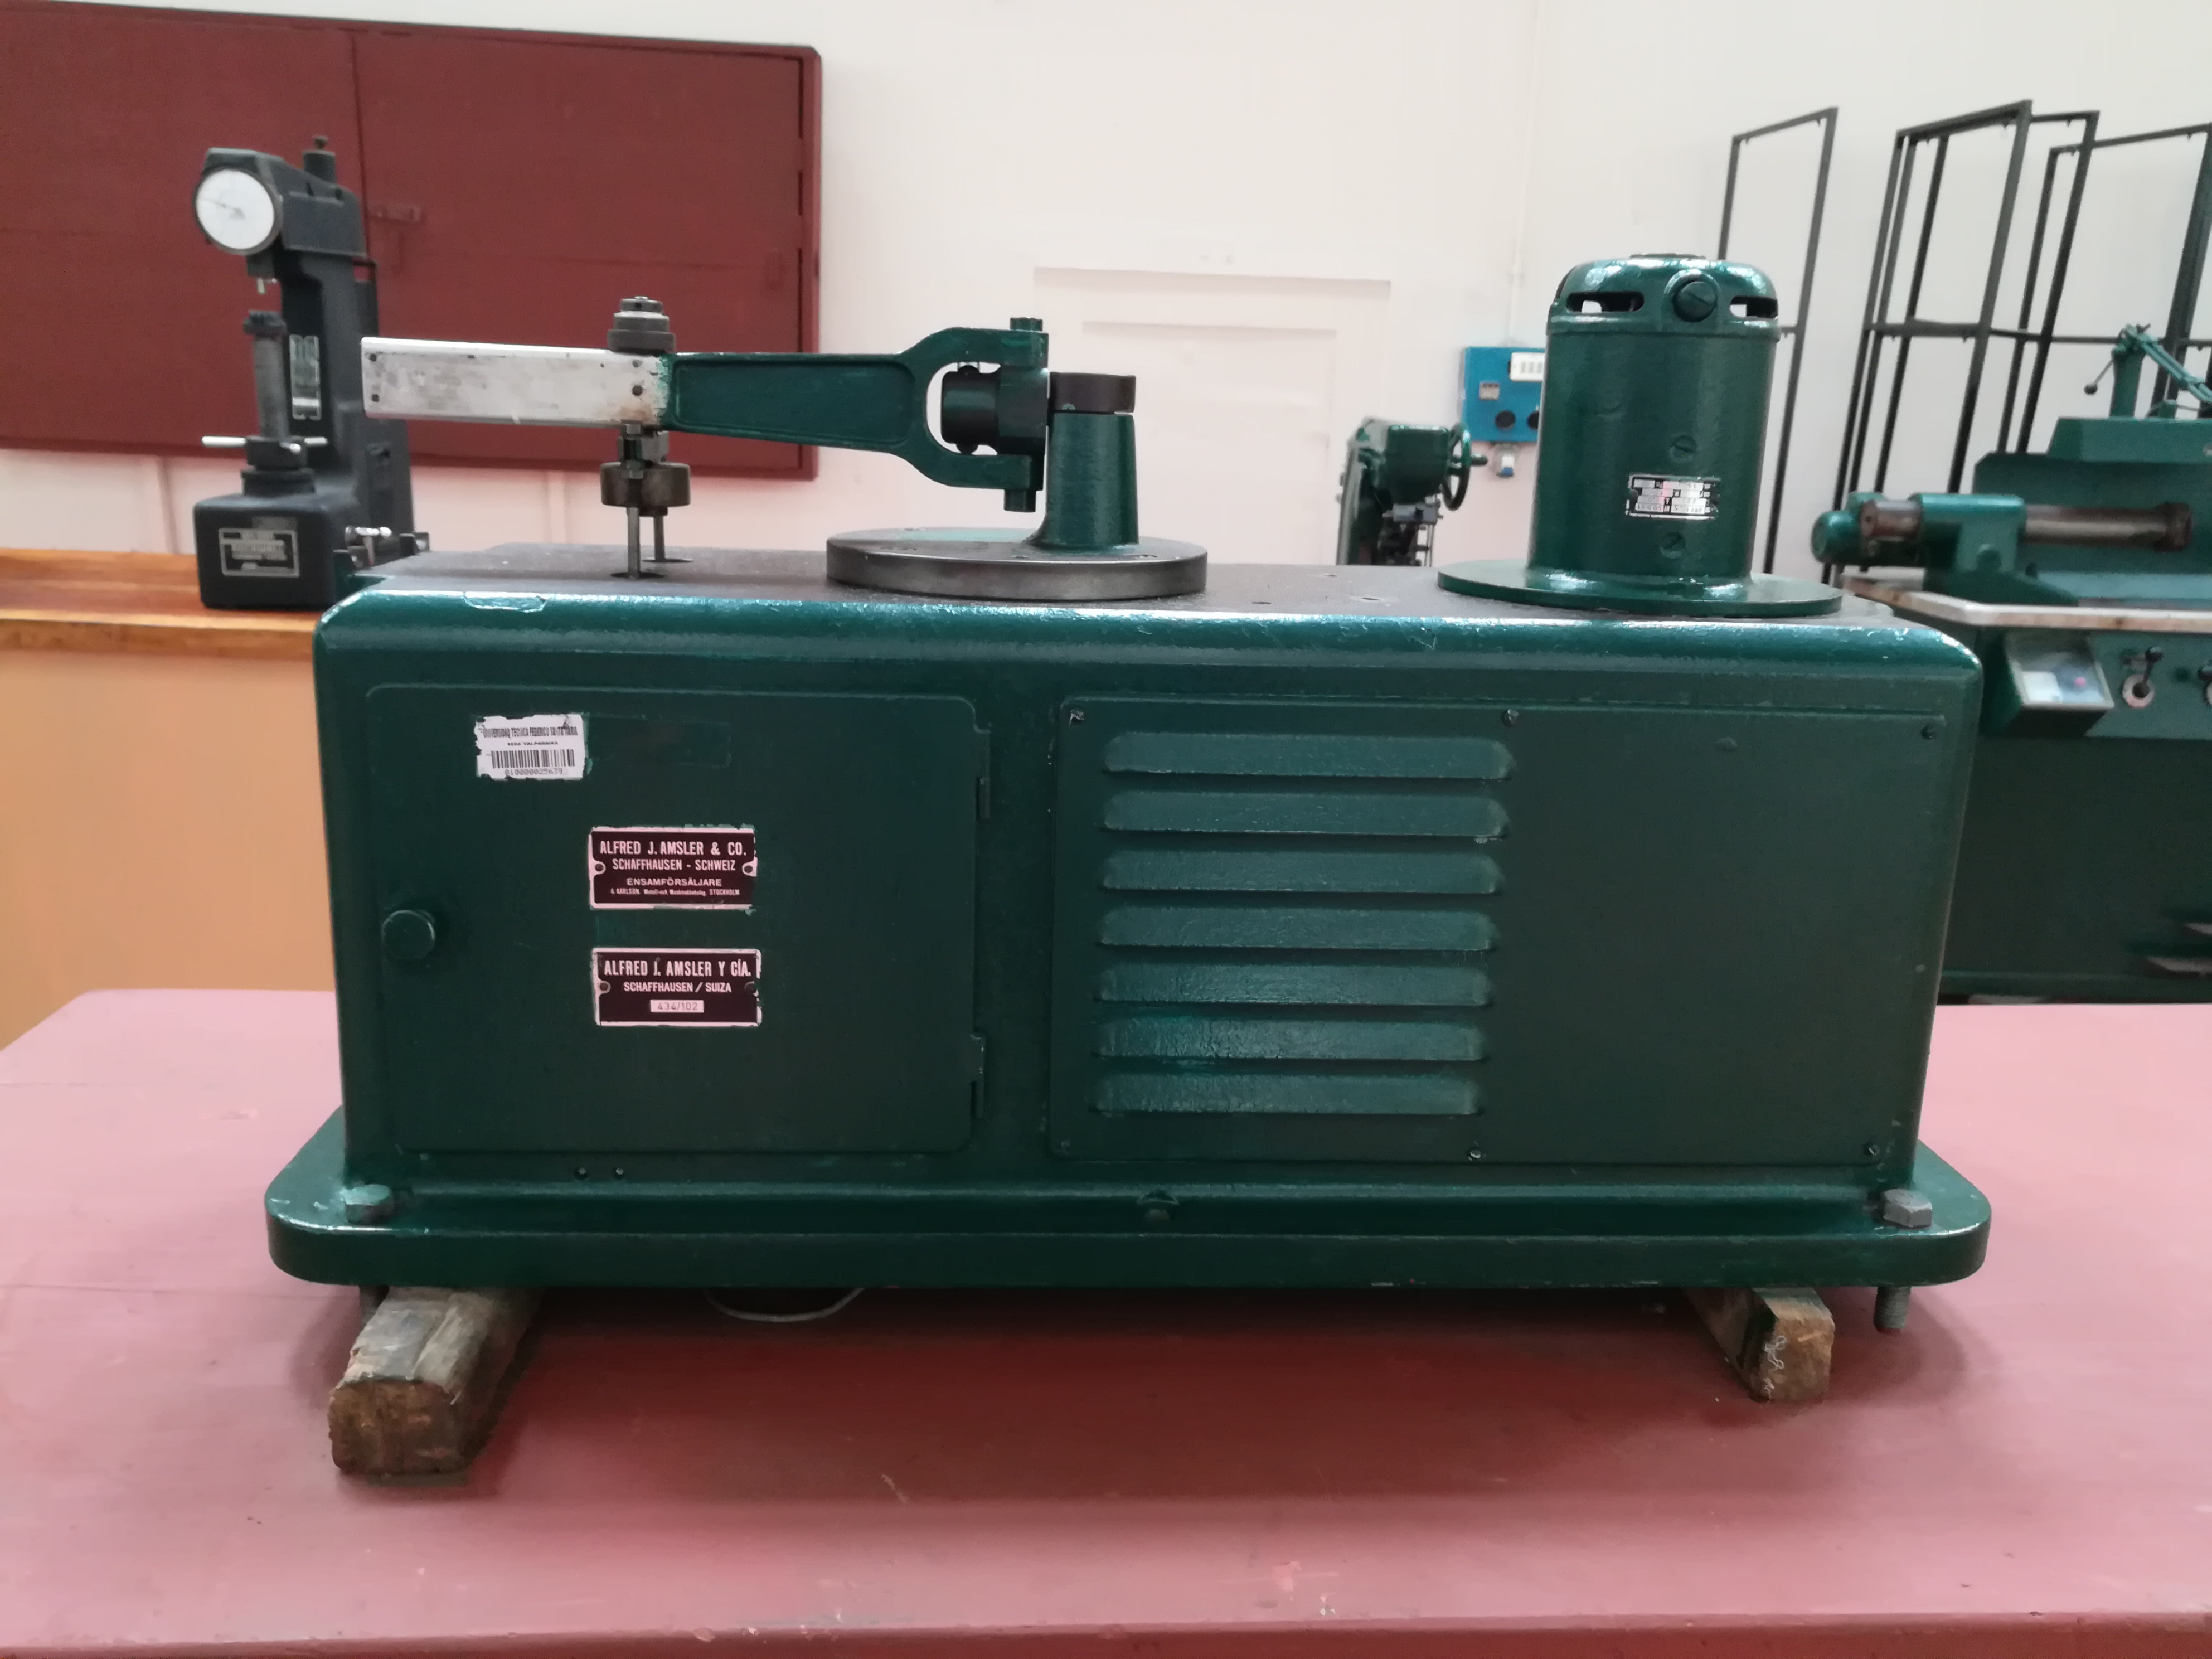
\includegraphics[width=1\linewidth]{Imagenes/maq_del.jpg}
		\caption{Vista delantera}\label{fig:maq_del}
	\end{subfigure}
	\begin{subfigure}{0.49\linewidth}
		\centering		
		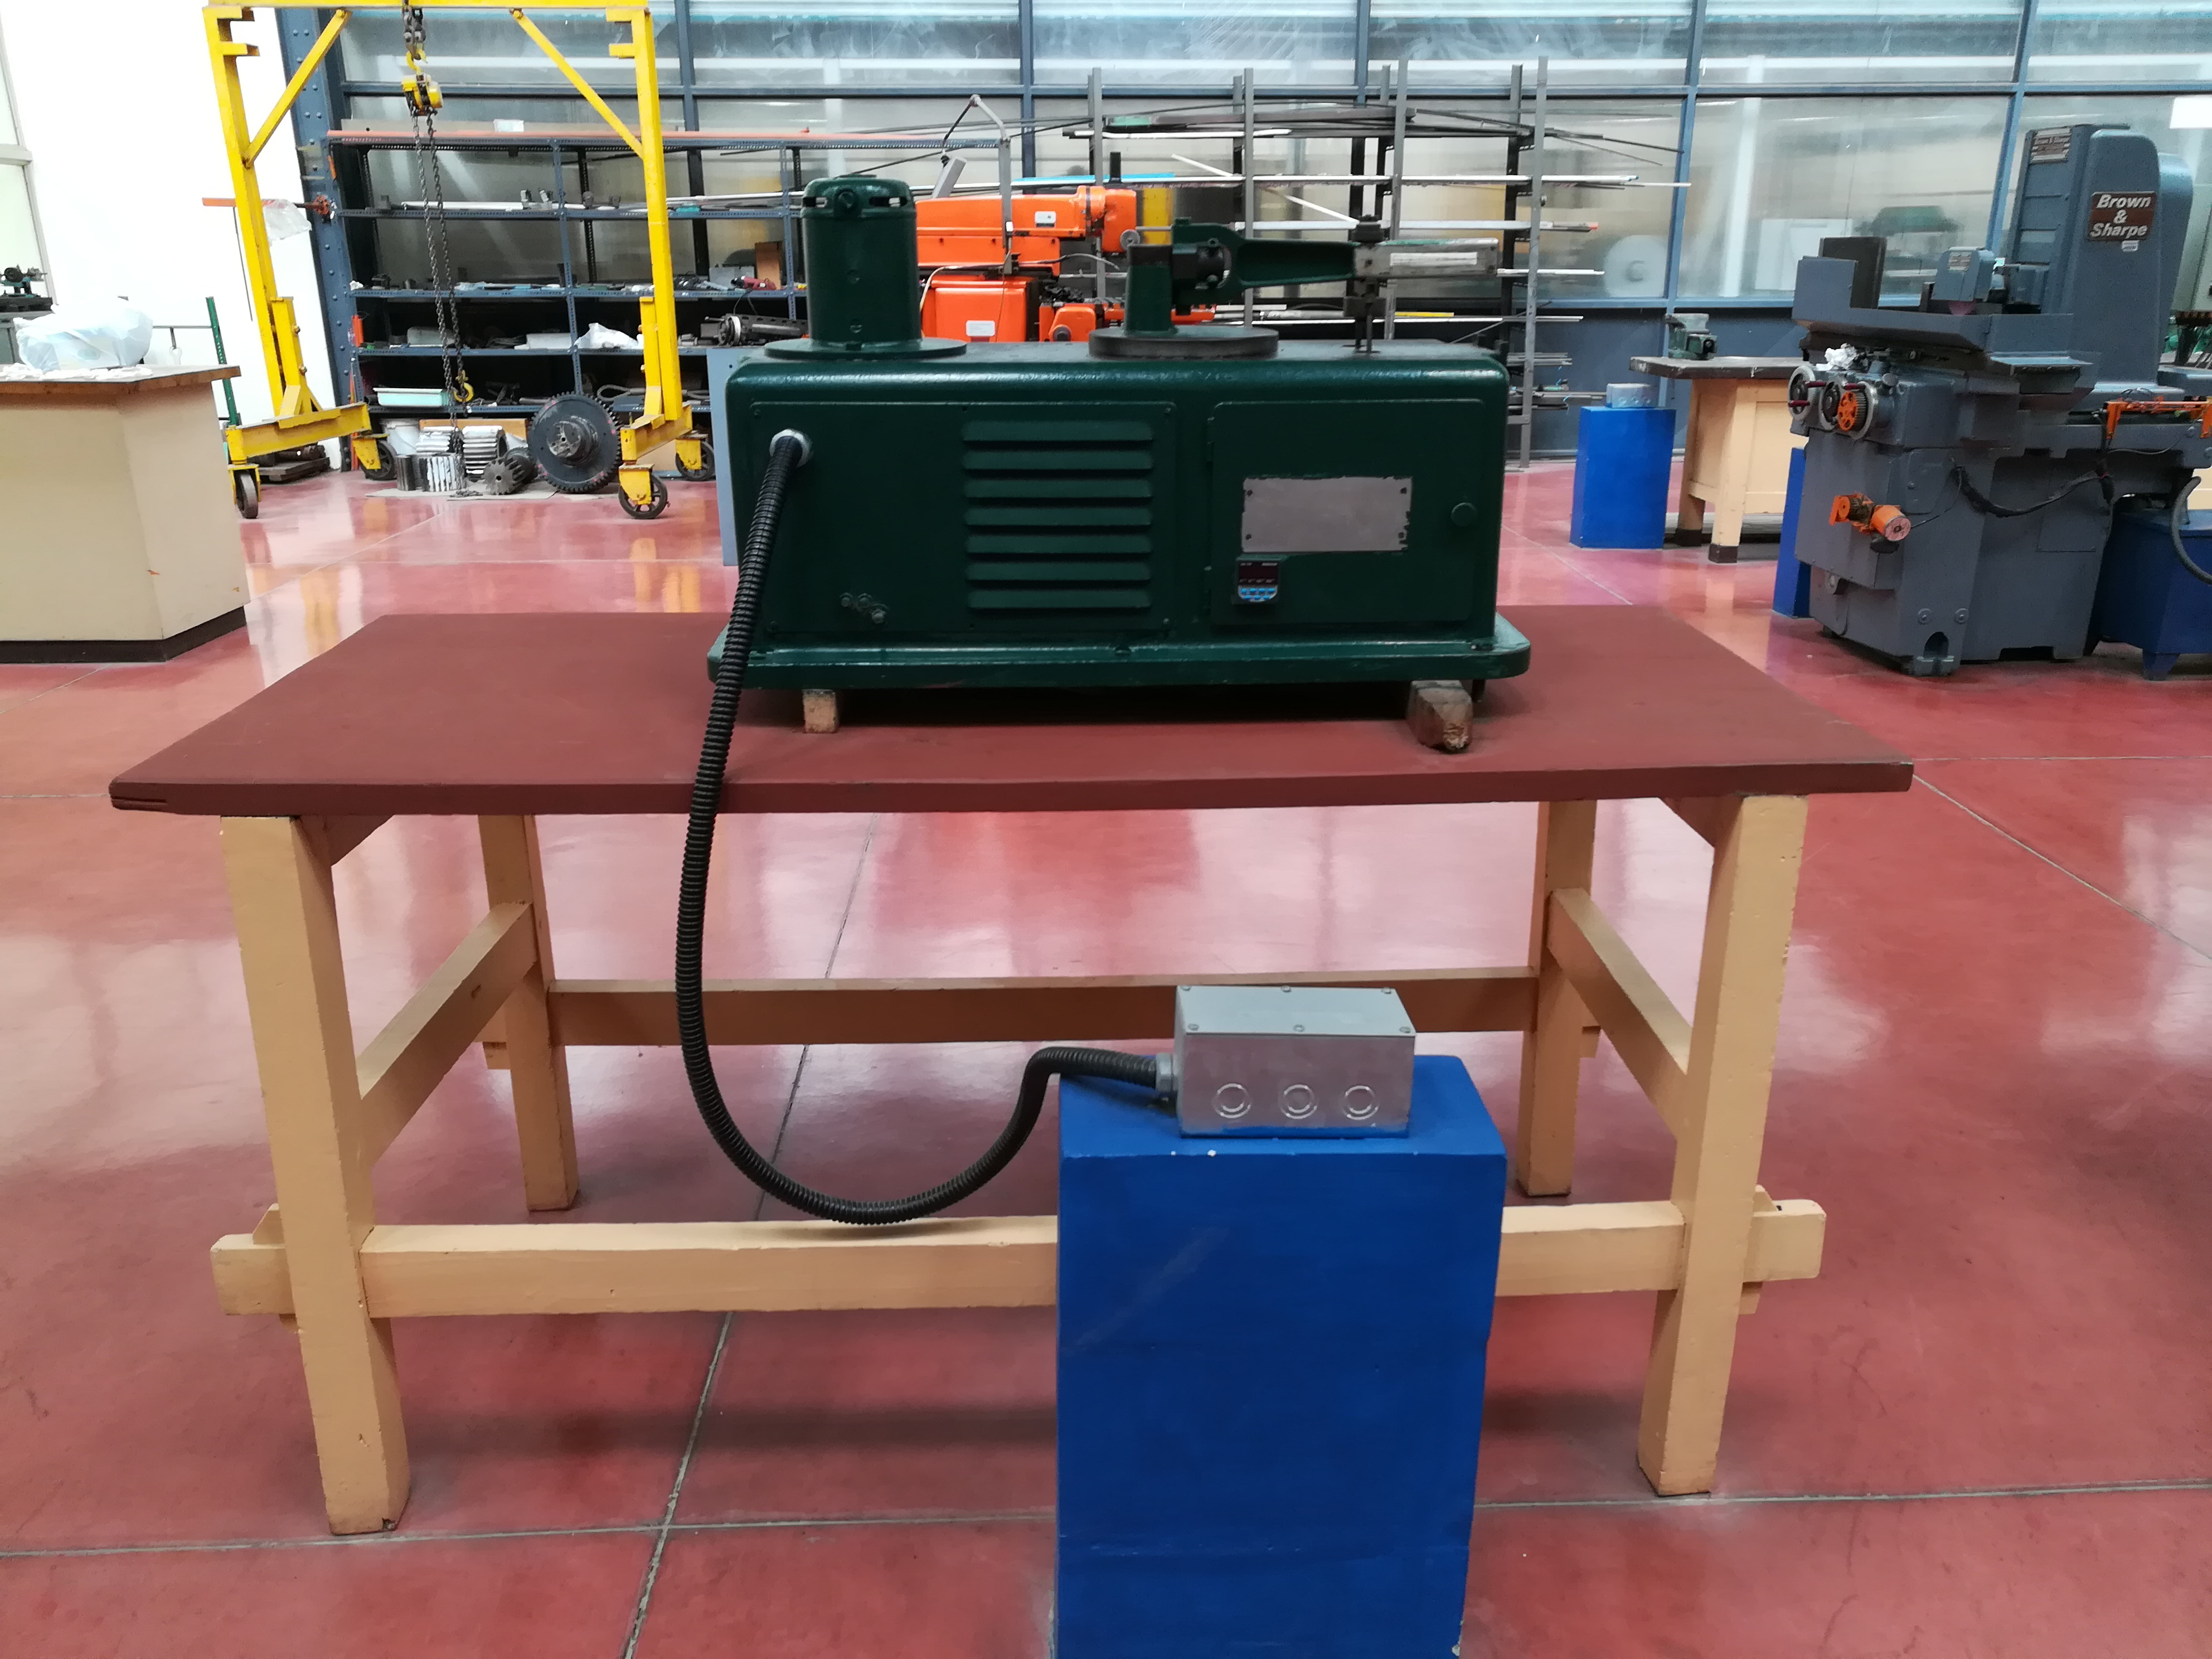
\includegraphics[width=1\linewidth]{Imagenes/maqfull_post.jpg}
		\caption{Vista posterior}\label{fig:maqfull_post}
	\end{subfigure}
	\begin{subfigure}{0.5\linewidth}
		\centering		
		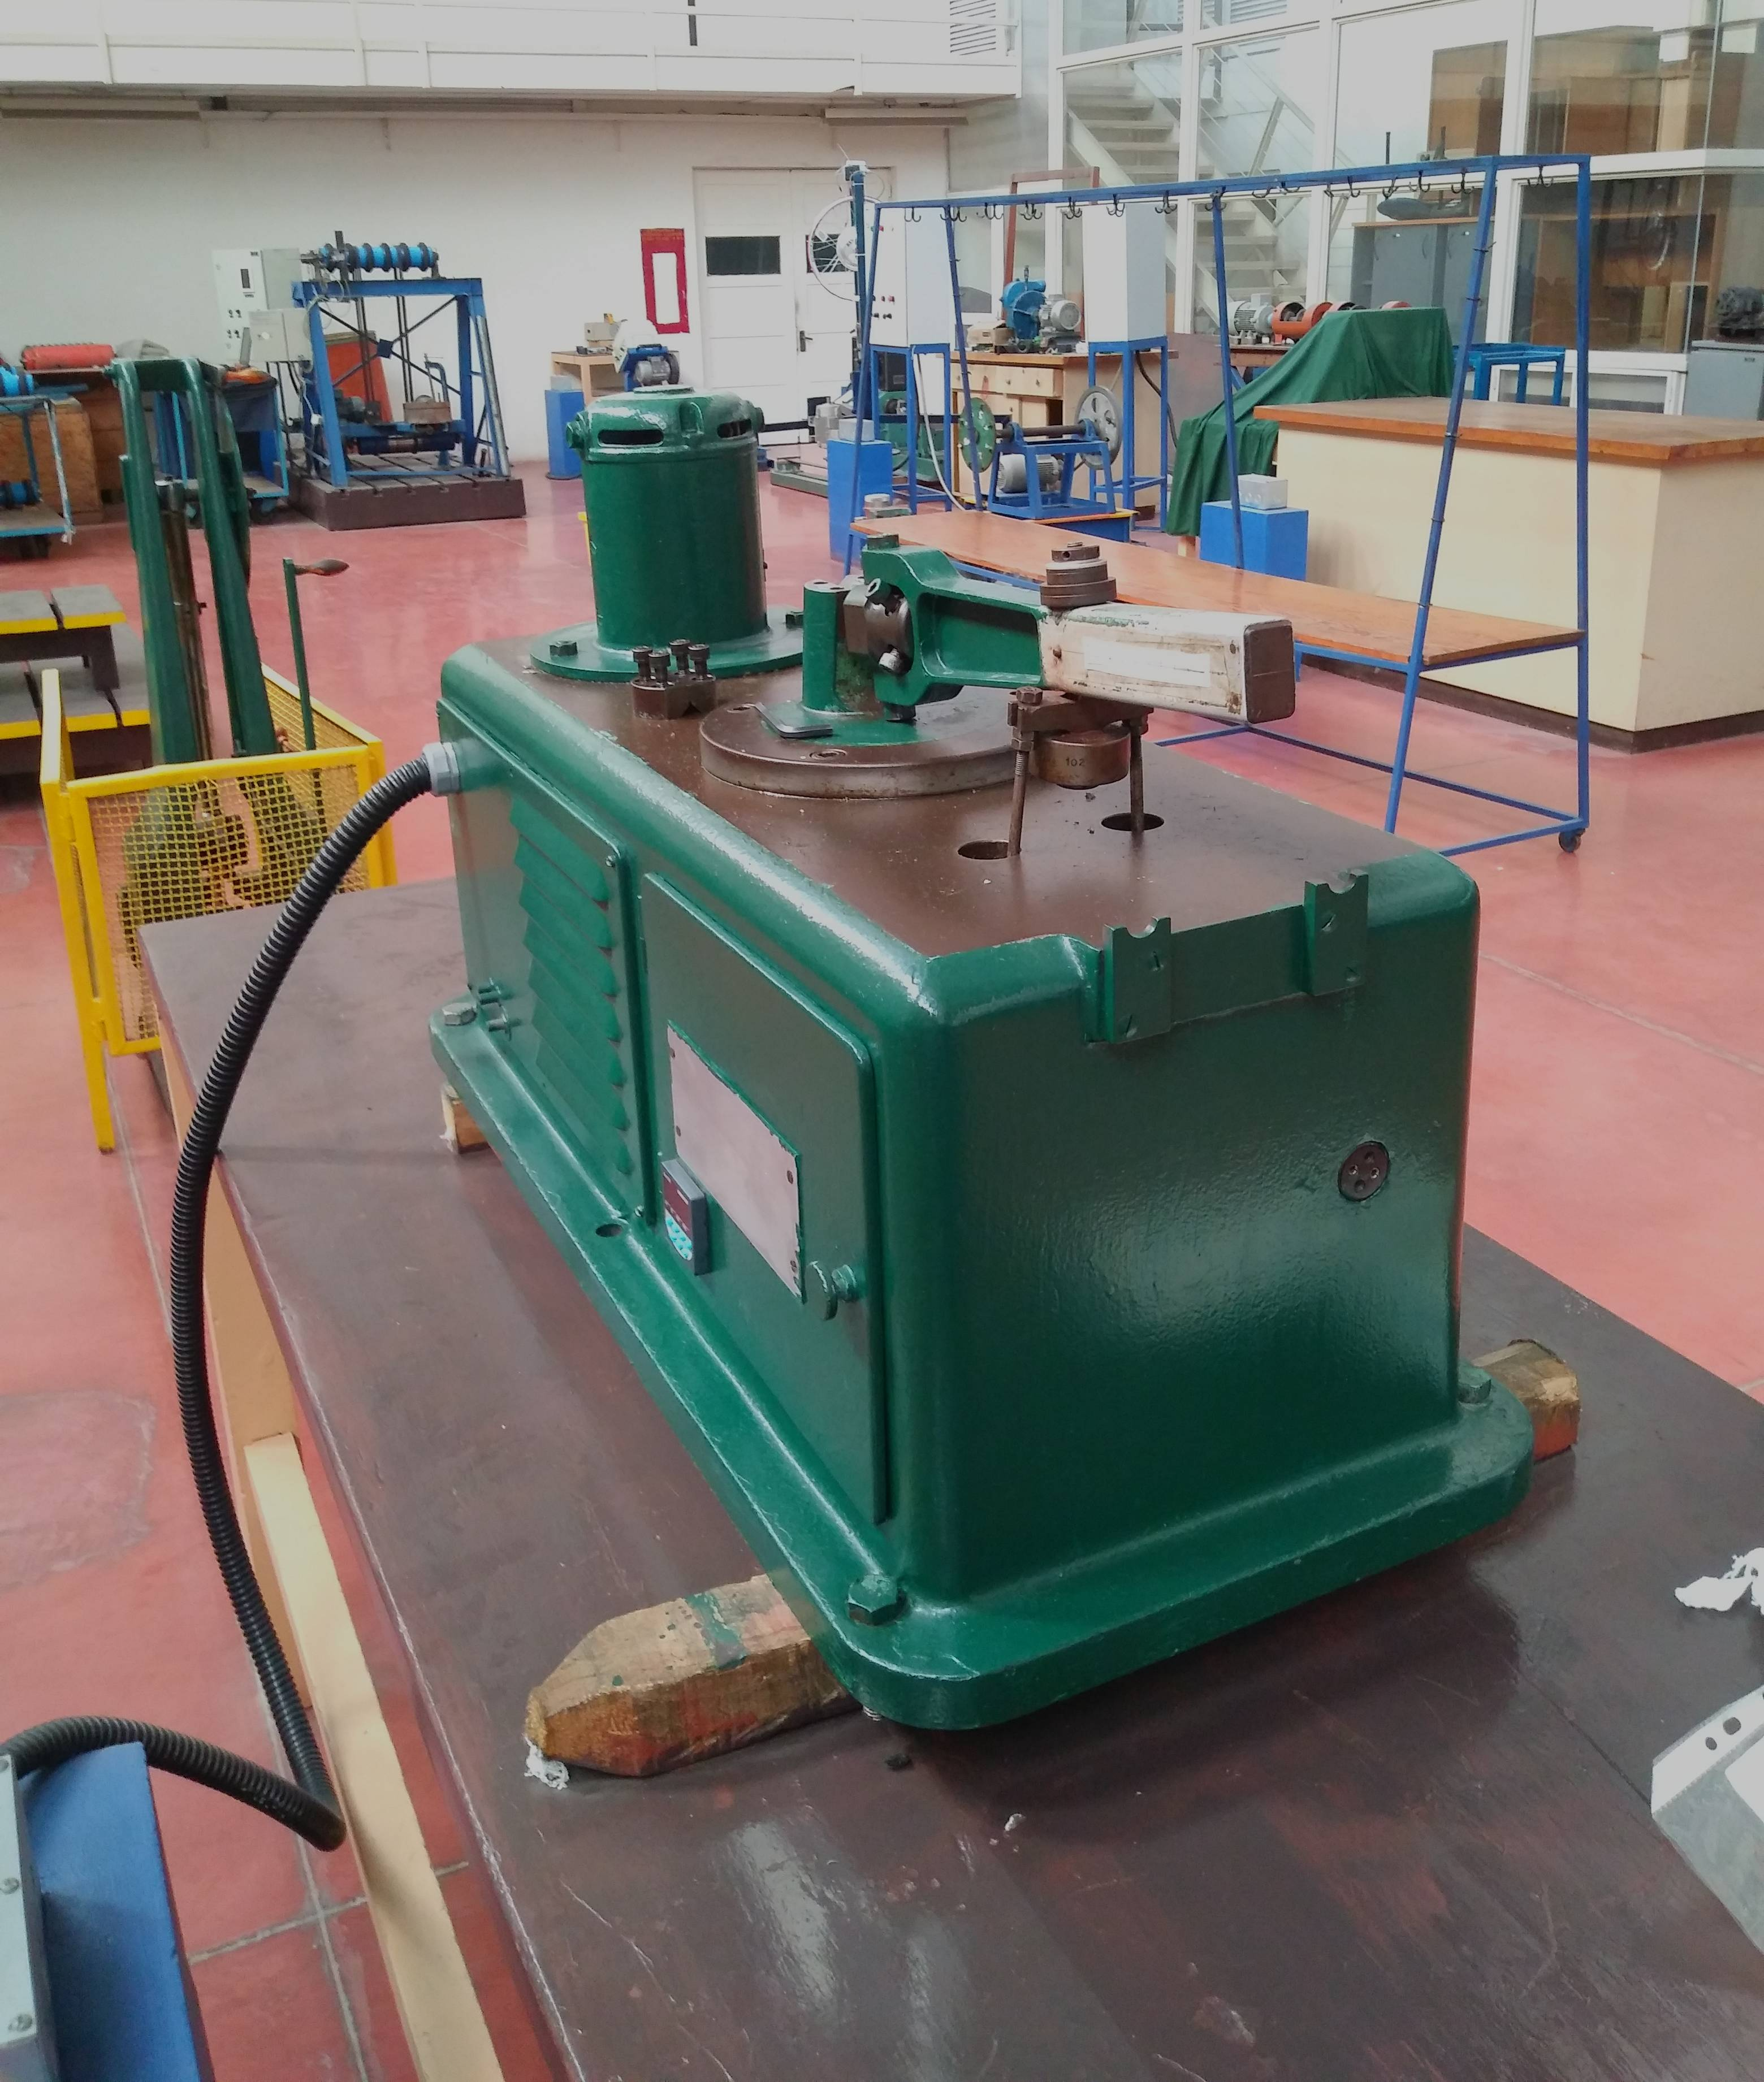
\includegraphics[width=0.8\linewidth]{Imagenes/maq_iso.jpg}
		\caption{Vista en perspectiva}\label{fig:maq_iso}		
	\end{subfigure}
\caption{Máquina de fatiga en flexión en el laboratorio de tecnología mecánica}
\label{fig:maq_fat}
\end{figure}

\newpage

\section{La madera como elemento constructivo}
La madera es un material de construcción simple y liviano, con ciertas características que lo vuelven particular respecto a otros materiales de construcción. Esto hace que al momento de trabajar con la madera se requiera un conocimiento especial y se tomen en consideración reglas específicas que permitan realizar diseños de calidad que aprovechen al máximo las propiedades y beneficios que provee.

Existen cientos de variedades de madera, donde cada una tiene propiedades distintas. Además, al haber sido parte de un organismo vegetal en crecimiento, hace que ninguna pieza de madera sea igual a otra y, dependiendo del tipo de corte, también varíen las propiedades mecánicas. Frente a esta importante variabilidad del material, surgen las normas en cada país que intentan delimitar y clasificar las distintas especies madereras que se encuentran en su región según el tipo de corte, contenido de humedad, su calidad o uso. Incluso, existen distintas metodologías de cálculo si se utiliza madera maciza, laminada encolada o aglutinada. En el caso de este trabajo, se utilizará exclusivamente madera maciza, por lo tanto, toda la metodología de cálculo e información respectiva a este tipo de madera, a excepción del pino radiata, se encuentra en la norma NCh 1198 Of. 1991 - Madera - Construcciones en madera - Cálculo.

\subsection{Anatomía de la madera}
La madera es un material que es fabricado naturalmente por los vegetales leñosos, con un alto grado de especialización y complejidad. Esto lo convierte en un material altamente heterogéneo, al estar especializado en llevar a cabo las funciones fundamentales del vegetal, lo que se ve reflejado en sus propiedades físicas y mecánicas. 

Una consecuencia de esta heterogeneidad es el comportamiento anisotrópico, teniendo un comportamiento distinto según la dirección en que se trabaja. Se establecen tres planos de referencia respecto a su propiedades físicas.
\begin{itemize*}
	\item Longitudinal: Sigue la misma dirección de la fibra o el eje del tronco.
	\item Radial: Pasa por el eje del tronco y es perpendicular a los anillos de crecimiento.
	\item Tangencial: Paralela a un plano tangente a los anillos de crecimiento.
\end{itemize*}
En relación a sus propiedades mecánicas se habla de dos direcciones, la paralela (longitudinal) y normal o perpendicular (englobando radial y tangencial). Esta diferencia hace que la madera sea capaz de soportar cargas de compresión de hasta 4 veces en dirección paralela respecto a la normal \cite{obe2002timber}. Esto quiere decir que siempre que sea posible, se deben instalar las piezas madereras para que resistan las cargas en su dirección longitudinal para un uso eficiente del material. De esta forma, se habla que las propiedades mecánicas de la madera son ortotrópicas.

Por último, es considerado un material higroscópico por su capacidad de captar o ceder agua del exterior, tanto en forma líquida como vapor. La cantidad de agua que contiene tenderá a estar en equilibrio con su entorno, lo que afectará sus propiedades físicas, mecánicas y en su posible degradación.

\subsection{Propiedades mecánicas de la madera}
Junto a la ortotropía de la madera, existen otras particularidades que influyen en sus propiedades, como la duración de la carga, el contenido de humedad y su calidad. En el primer caso, dado su carácter orgánico, es susceptible a degradarse por elementos externos como la lluvia, hongos, insectos o el sol, la cual se protege utilizando tratamientos químicos, e internos, que se cuantifica a través de un factor de modificación por duración de carga. En el segundo caso, a mayor cantidad de humedad la resistencia comienza a decaer, como también sus dimensiones se comienzan a modificar, afectando las uniones o ensambles. En último término, la calidad se reflejada en la cantidad de nudos, desviaciones de fibra o gemas que influyen en su comportamiento.

La tracción y compresión tienen resistencias distintas, además de las diferencias existentes entre las cargas paralelas y perpendiculares a la madera. La resistencia a la tracción paralela es comúnmente más alta que la compresión paralela, en la cual se debe calcular además la inestabilidad lateral. En el caso de la compresión y tracción perpendicular, los valores de resistencia son considerablemente más bajos, llegando a ser 9 y 20 veces menos resistente que su par paralelo, respectivamente. Esto se debe a la eficiencia de construcción de los árboles al no estar solicitados fuertemente en estas direcciones. 

Esta diferencia de resistencia y comportamiento entre la tracción y compresión de la madera implica que en el cálculo de la flexión se deban separar las zonas flexo-comprimidas y flexo-traccionadas, a pesar que la resistencia a la flexión de una madera sea única. Por otro lado, el esfuerzo cortante en un elemento de madera puede tener diversos modos:
\begin{itemize*}
	\item Cortadura: las fibras son cortadas transversalmente.
	\item Deslizamiento: las fibras se desplazan longitudinalmente.
	\item Rodadura: las fibras se desplazan una sobre otra.
\end{itemize*}
Donde la rotura se produce por deslizamiento al ser el plano más débil \cite{steiger2017basics}.

En última instancia, la resistencia a la fatiga de la madera es muy buena en comparación a otros materiales estructurales con estructura cristalina como el acero \cite{sanchez2014guia}, siendo resistente a la acción cíclica de las cargas y al amortiguamiento de estas. 

\section{Acero}
El acero es una aleación basada principalmente en fierro y carbono, pudiendo tener concentraciones de otros elementos incluso. Sus propiedades mecánicas son fuertemente sensitivas al contenido de carbono, por lo que muchas veces es clasificado a partir de su porcentaje, como aceros de bajo, media y alto en carbono. También inciden en sus propiedades mecánicas las características de fabricación y si reciben algún tipo de tratamiento térmico \cite{callister2001fundamentals}.

La probeta utilizada en la máquina de fatiga se fabrica actualmente de acero de bajo carbono, los cuales bajo nomenclatura AISI/SAE se denominan 1020 y 1040, es decir, son aceros que sólo contienen concentraciones residuales de otros elementos distintos al carbono y su concentración es del 0,20\% y 0,40\% respectivamente. Los aceros de bajo carbono se caracterizan por ser más débiles, pero con una alta tenacidad. Además, son maquineables, soldables y más baratos respecto a otros tipos de aceros.

Para la mayoría de los aceros, su comportamiento bajo carga se divide en una zona elástica y otra plástica, como se muestra en la fig. \ref{fig:esf-def_curve}. La zona elástica se caracteriza por tener un módulo de elasticidad $E$, que en el caso de los aceros ronda entre 200 y 210 GPa. La transición de la zona elástica a plástica es gradual y comienza cuando deja de existir una relación lineal entre los esfuerzos y la deformación, es decir, llega al esfuerzo de fluencia, $\sigma_y$. Una vez en la región de deformación plástica el punto de esfuerzo máximo en una curva ingenieril de esfuerzo-deformación es llamado esfuerzo último, $\sigma_u$ \cite{beer2010mecanica}.

\begin{figure}[h!]
\centering
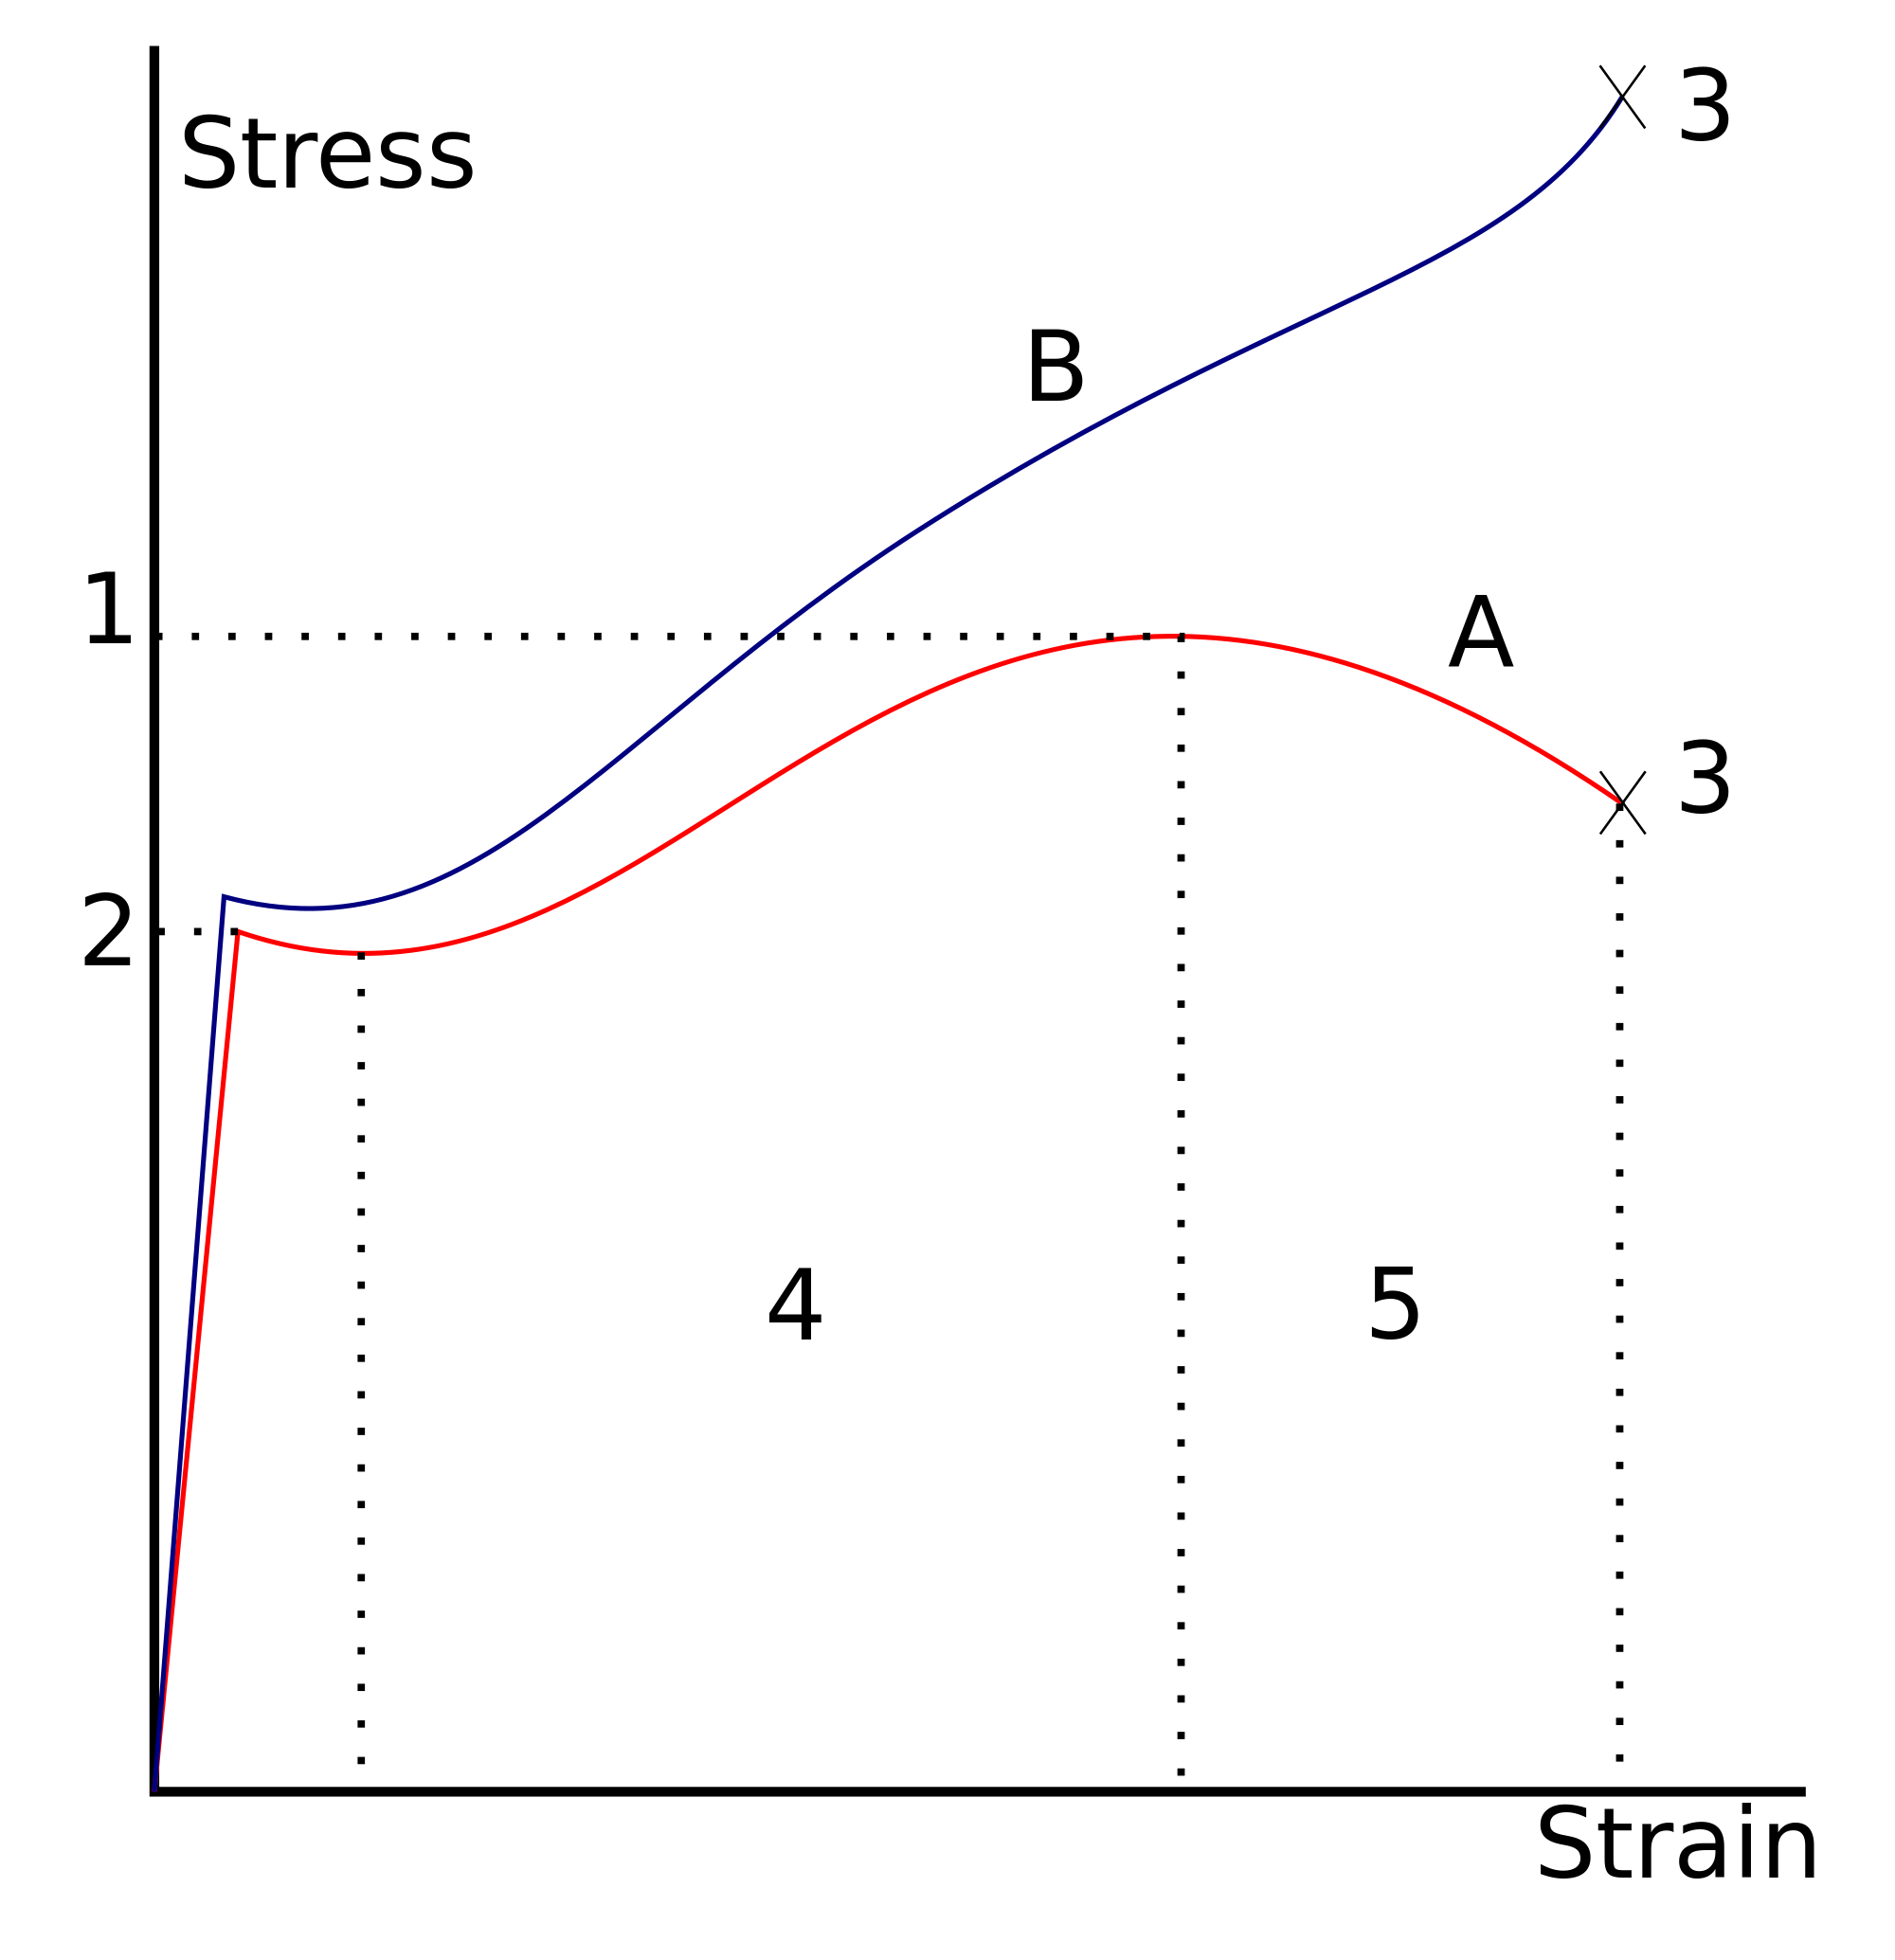
\includegraphics[width=0.5\linewidth]{Imagenes/strain-stress_curve.png}
\caption{Curva de esfuerzo-deformación ingenieril (A) y real (B) de un acero. Los puntos representan: (1) Esfuerzo último ($\sigma_u$), (2) esfuerzo de fluencia ($\sigma_y$), (3) esfuerzo de ruptura, (4) región de endurecimiento por deformación y (5) región de estricción. \cite{richfield}}
\label{fig:esf-def_curve}
\end{figure}

\newpage

\section{Software de simulación de elementos finitos}

En el desarrollo de esta tesis se utiliza el software de elementos finitos ANSYS para la simulación estática de la probeta y el software Autodesk Inventor para la simulación de la estructura soportante en su módulo de análisis de esfuerzos (\textit{Stress Analysis}).

En el caso de ANSYS, se utilizó el ambiente ``\textit{Static Structural}'', el cual determina los desplazamientos, esfuerzos y fuerzas en la estructura que está sometida a una o varias cargas. Además permite el análisis elastoplástico de un material, siendo utilizado el modelo de plasticidad multilineal de endurecimiento isotrópico (\textit{Multilinear Isotropic Hardening} o MISO). 

Inventor, por otro lado, el módulo de análisis de esfuerzos puede realizar análisis de tipo estático, para evaluar las condiciones de carga de la estructura, y de tipo modal, para evaluar los modos de frecuencia natural de la estructura.


